\documentclass[11pt,class=report,crop=false]{standalone}
\usepackage[screen]{../mathgame}

% Commenter pour afficher les figures longuettes à calculer !!
%\renewcommand{\commentfigure}[1]{\mybox{\emph{Ici une figure.}}}  % sans les figures compliquées

\begin{document}


%====================================================================
\chapitre{Trigonométrie}
%====================================================================


\insertvideo{uDqBddWEuhg}{partie 1.1. Sinus, cosinus, tangente}

\insertvideo{u7b6gpg1DIo}{partie 1.2. Coordonnées polaires, cylindriques, sphériques}

\objectifs{Savoir mesurer et calculer les angles est fondamental !}


%%%%%%%%%%%%%%%%%%%%%%%%%%%%%%%%%%%%%%%%%%%%%%%%%%%%%%%%%%%%%%%%%%%%%
\section{Sinus, cosinus, tangente}

%--------------------------------------------------------------------
\subsection{Cercle trigonométrique}

\index{cercle trigonmetrique@cercle trigonométrique}

Le cercle trigonométrique est le cercle centré à l'origine et de rayon $1$.
Il est orienté dans le sens trigonométrique (le sens inverse des aiguilles d'une montre) à partir du point $(1,0)$. Sur le cercle ci-dessous, on a placé quelques points avec les angles correspondants en radians (de $0$ à $2 \pi$) et en degrés (de $\ang{0}$ à $\ang{360}$) ainsi que leurs coordonnées $(x,y)$.
 
\myfigure{0.6}{\tikzinput{fig-trigo-01}}


\index{angle!degres@degrés}
\index{angle!radians}

La conversion entre les angles en degrés et en radians se fait par les formules suivantes :

$$\theta_{\text{radian}} = 2\pi \frac{\theta_{\text{degré}}}{360}$$
et
$$\theta_{\text{degré}} = 360 \frac{\theta_{\text{radian}}}{2\pi}.$$

Dans ce cours, nous utiliserons principalement le radian comme unité de mesure des angles.


%--------------------------------------------------------------------
\subsection{Sinus, cosinus, tangente}


Le point $M$ du cercle trigonométrique correspondant à l'angle $\theta$ a pour coordonnées $(\cos(\theta),\sin(\theta))$.
Autrement dit, l'abscisse de $M$ est $\cos(\theta)$ et l'ordonnée de $M$ est $\sin(\theta)$.


\myfigure{0.7}{\tikzinput{fig-trigo-02}}

Pour tout $\theta$ n'appartenant pas à $\{\ldots, -\frac\pi2, \frac\pi2, \frac{3\pi}{2}, \frac{5\pi}{2},\ldots  \}$
la tangente est définie par
$$\tan(\theta) = \frac{\sin(\theta)}{\cos(\theta)}.$$

La droite $(OM)$ coupe la droite d'équation $(x=1)$ en $T$,
l'ordonnée du point $T$ est $\tan(\theta)$.

Voici les valeurs des sinus et cosinus pour les angles remarquables.

\begin{center}
\begin{minipage}{0.4\textwidth}
{
\renewcommand{\arraystretch}{2.5}
$$\small 
\begin{array}{c|*{5}{c}}
	x     & \hphantom{X} 0 \hphantom{X} & \hphantom{X} \dfrac\pi6 \hphantom{X} &  \hphantom{X} \dfrac\pi 4 \hphantom{X}
	& \hphantom{X} \dfrac \pi 3 \hphantom{X} & \hphantom{X} \dfrac \pi 2 \hphantom{X} \\
	\hline
	\cos(x)   & 1 & \dfrac{\sqrt3}{2} & \dfrac{\sqrt2}{2} & \dfrac12 & 0 \\
	\hline
	\sin(x)   & 0 &\dfrac12 & \dfrac{\sqrt2}{2} & \dfrac{\sqrt3}{2} & 1\\
	\hline
	\tan(x)   & 0 & \dfrac{1}{\sqrt{3}} & 1 & \sqrt{3} &
\end{array}
$$
}
\end{minipage}\qquad\qquad\qquad
\begin{minipage}{0.4\textwidth}
\myfigure{0.9}{\tikzinput{fig-trigo-03}}
\end{minipage}
\end{center}


Les formules de base avec sinus et cosinus sont :
\begin{center}
\begin{minipage}{0.4\textwidth}
\begin{align*}
	& \cos^2(x) + \sin^2(x) = 1 \\
	& \cos(x+2\pi)=\cos(x) \\
	& \sin(x+2\pi)=\sin(x) \\
\end{align*}
\end{minipage}\qquad
\begin{minipage}{0.4\textwidth}
\begin{align*}
	\cos (-x) &= \cos(x) \\
	\sin (-x) &= -\sin(x) \\
\end{align*}
\end{minipage}
\end{center}

Il en existe beaucoup d'autres !

%--------------------------------------------------------------------
\subsection{Fonctions}

La fonction cosinus $x \mapsto \cos(x)$ est périodique de période $2\pi$
et elle est paire (donc symétrique par rapport à l'axe des ordonnées).
La fonction sinus $x \mapsto \sin(x)$ est aussi périodique de période de $2\pi$ mais elle est impaire (donc symétrique par rapport à l'origine).


\myfigure{0.65}{
	\tikzinput{fig-trigo-04}
}

Voici un zoom sur l'intervalle $[-\pi,\pi]$.
\myfigure{1.2}{
	\tikzinput{fig-trigo-05}
}



La fonction $x \mapsto \tan(x)$ est périodique de période $\pi$ ; c'est une fonction impaire.

\myfigure{0.55}{
	\tikzinput{fig-trigo-06}
}


Voici les dérivées:
\begin{align*}
	\cos'(x)&= -\sin(x)\\
	\sin'(x)&=\cos(x)\\
	\tan'(x) &= 1+\tan^2(x)=\frac{1}{\cos^2(x)}\\
\end{align*}


%%%%%%%%%%%%%%%%%%%%%%%%%%%%%%%%%%%%%%%%%%%%%%%%%%%%%%%%%%%%%%%%%%%%%
\section{Arcsinus, arccosinus, arctangente}


Les fonctions trigonométriques inverses permettent de retrouver un angle connaissant la valeur du sinus (ou du cosinus ou de la tangente).

%---------------------------------------------------------------
\subsection{Arcsinus}

Considérons la fonction $\sin : \Rr \to [-1,1]$, $x \mapsto \sin(x)$.
Pour obtenir une bijection à partir de cette fonction, il faut considérer la restriction
de sinus à l'intervalle $[-\frac\pi2,\frac\pi2]$. Sur cet intervalle, la fonction sinus est continue et strictement croissante, donc la restriction
$$\sin_| : [-\tfrac\pi2,+\tfrac\pi2] \to [-1,1]$$
est bijective.
Sa bijection réciproque s'appelle la fonction \defi{arcsinus} :
$$\arcsin : [-1,1] \to [-\tfrac\pi2,+\tfrac\pi2]$$


\begin{center}
\begin{minipage}{0.55\textwidth}
\myfigure{1}{\tikzinput{fig-trigo-07}}	
\end{minipage}\qquad
\begin{minipage}{0.35\textwidth}
\myfigure{1}{\tikzinput{fig-trigo-08}}	
\end{minipage}
\end{center}
		

On a donc, par définition de la bijection réciproque :
$$
\begin{array}{cl}
	\displaystyle \sin\bigl(\arcsin(x)\bigr) = x &  \qquad (x \in [-1,1])\\
	\displaystyle \arcsin\bigl(\sin(x)\bigr) = x &  \qquad (x \in [-\frac\pi2,+\frac\pi2]) \\
\end{array}
$$
	
Autrement dit :
$$\text{Si } \quad  x\in \left[-\frac\pi2,+\frac\pi2\right] \qquad \sin(x)=y \iff x = \arcsin(y)$$

Terminons avec la dérivée de $\arcsin$ :
$$\arcsin'(x) = \frac{1}{\sqrt{1-x^2}} \qquad\qquad (x \in ]-1,1[)$$

%---------------------------------------------------------------
\subsection{Arccosinus}


La restriction $\cos_| : [0,\pi] \to [-1,1]$
est une bijection. Sa bijection réciproque est la fonction \defi{arccosinus} :
$$\arccos : [-1,1] \to [0,\pi]$$

\begin{center}
\begin{minipage}{0.55\textwidth}	
\myfigure{1}{\tikzinput{fig-trigo-09}}
\end{minipage}\qquad
\begin{minipage}{0.35\textwidth}
\myfigure{1}{\tikzinput{fig-trigo-10}}
\end{minipage}
\end{center}

$$
\begin{array}{cl}
	\displaystyle \cos\bigl(\arccos(x)\bigr) = x &  \qquad (x \in [-1,1])\\
	\displaystyle \arccos\bigl(\cos(x)\bigr) = x &  \qquad (x \in [0,\pi]) \\
\end{array}
$$


$$\text{Si } \quad x\in [0,\pi] \qquad \cos(x)=y \iff x = \arccos(y)$$

$$\arccos'(x) = \frac{-1}{\sqrt{1-x^2}} \qquad\qquad (x \in {}]-1,1[)$$

%---------------------------------------------------------------
\subsection{Arctangente}

La restriction $\tan_| : {}]-\tfrac\pi2,+\tfrac\pi2[ \to \Rr$
est une bijection.
Sa bijection réciproque est la fonction \defi{arctangente}\index{arctangente} :
$$\arctan : \Rr \to {}]-\tfrac\pi2,+\tfrac\pi2[$$

\begin{center}
	\begin{minipage}{0.45\textwidth}
	\myfigure{0.45}{\tikzinput{fig-trigo-11}}	
	\end{minipage}\qquad
	\begin{minipage}{0.35\textwidth}
	\myfigure{0.5}{\tikzinput{fig-trigo-12}}	
	\end{minipage}
\end{center}



$$
\begin{array}{cl}
	\displaystyle \tan\bigl(\arctan(x)\bigr) = x &  \qquad (x \in \Rr)\\
	\displaystyle \arctan\bigl(\tan(x)\bigr) = x &  \qquad (x \in {}]-\frac\pi2,+\frac\pi2[) \\
\end{array}
$$

$$\text{Si } \quad x\in \left]-\frac\pi2,+\frac\pi2\right[ \qquad \tan(x)=y \iff x = \arctan y$$


$$\arctan'(x) = \frac{1}{1+x^2} \qquad \qquad (x \in \Rr)$$

%--------------------------------------------------------------------
\subsection{La fonction arctan2}

\index{arctan2} 
 
Détaillons le fonctionnement de la fonction $\arctantwo$ qui est essentielle en programmation, mais rarement expliquée dans les cours de mathématiques. L'objectif est tout simplement de retrouver l'angle $\theta$ du point $M$ de coordonnées $(x,y)$ (plus précisément l'angle entre $\vec i$ qui dirige l'horizontale et $\vec{OM}$).

\myfigure{1}{\tikzinput{fig-arctan2-01}}

Le cas fondamental est lorsque le point $M(x,y)$ est situé dans le premier quadrant ($x >0$ et $y\ge0$) alors :
$$\tan(\theta) = \frac{y}{x},$$ 
donc
$$\theta = \arctan \left( \frac y x \right).$$

Il faut adapter le calcul lorsque $M(x,y)$ appartient aux autres quadrants, c'est ce que fait la fonction $\arctantwo(y,x)$ (attention à l'ordre des variables!).
La fonction $\arctantwo(y,x)$ est définie pour tout $(x,y) \neq (0,0)$ et renvoie l'angle $\theta \in ]-\pi,\pi]$ associé au point $M$ avec un angle positif pour les points au-dessus de l'axe des abscisses et un angle négatif en-dessous.


\myfigure{0.5}{\tikzinput{fig-arctan2-02}}


La valeur $\arctantwo(y,x)$ se calcule en fonction de $\arctan \left| \frac y x \right|$, où $\left| \frac y x \right|$ est la valeur absolue de $\frac{y}{x}$, selon le schéma ci-dessous :

\myfigure{0.7}{\tikzinput{fig-arctan2-03}}

Voici la définition de $\arctantwo(y,x)$ à l'intérieur de chacun des quatre quadrants :
$$\arctantwo(y,x) = 
\begin{cases}
\arctan\left| \frac y x \right| & \text{ si } x>0, y>0 \\
-\arctan\left| \frac y x \right| \ + \pi & \text{ si } x<0, y>0 \\
-\arctan\left| \frac y x \right| & \text{ si } x>0, y<0 \\
\arctan\left| \frac y x \right| \ -\pi & \text{ si } x<0, y<0 \\	
\end{cases}$$


Sur les axes :
$$
\begin{cases}
\arctantwo(0,x) = 0    & \text{ si } x>0 \\
\arctantwo(0,x) = \pi  & \text{ si } x<0 \\
\arctantwo(y,0) = \frac\pi2  & \text{ si } y>0 \\
\arctantwo(y,0) = -\frac\pi2  & \text{ si } y<0 \\	
\end{cases}$$
On rappelle que la fonction n'est pas définie en $(0,0)$.
Par définition la fonction $\arctantwo$ renvoie un angle $\theta$ appartenant à $]-\pi,+\pi]$. On peut facilement obtenir un angle de l'intervalle $[0,2\pi[$ : si $\theta < 0$, on change $\theta$ en $\theta+2\pi$.


%%%%%%%%%%%%%%%%%%%%%%%%%%%%%%%%%%%%%%%%%%%%%%%%%%%%%%%%%%%%%%%%%%%%%
\section{Coordonnées polaires}

\index{coordonnees@coordonnées!polaires}

Plutôt que de repérer un point du plan $\Rr^2$ par ses coordonnées cartésiennes $(x,y)$, on peut le faire au moyen de sa distance à l'origine et de l'angle formé avec l'horizontale : ce sont les coordonnées polaires.


%----------------------------------------------------
\subsection{Définition}

Soit $M$ un point du plan $\Rr^2$. Soit $O=(0,0)$ l'origine. Soit $(O, \vec i, \vec j)$ un repère orthonormé direct.

\begin{itemize}
	\item On note $r = \| \overrightarrow{OM} \|$, la distance de $M$ à l'origine.
	\item On note $\theta$ l'angle entre $\vec i$ et $\overrightarrow{OM}$.
\end{itemize}

\myfigure{1}{\tikzinput{fig-trigo-13}}

On note $[r:\theta]$ les \defi{coordonnées polaires} du point $M$. Dans ce cours, $r$ sera positif.
L'angle n'est pas déterminé de manière unique, plusieurs choix sont possibles. Pour avoir l'unicité, on peut limiter $\theta$ à l'intervalle $]-\pi,+\pi]$, ou bien $[0,2\pi[$. On n'attribue généralement pas de coordonnées polaires au point origine (l'angle n'aurait pas de sens). 


%--------------------------------------------------------------------
\subsection{Conversion}

\bigskip
\evidence{Coordonnées polaires vers coordonnées cartésiennes.}

On retrouve les coordonnées cartésiennes $(x,y)$ à partir des coordonnées polaires $[r:\theta]$ par les formules
$$x = r\cos(\theta) \qquad\text{ et }\qquad y = r \sin(\theta).$$


\bigskip
\evidence{Coordonnées cartésiennes vers coordonnées polaires.}

On retrouve  $r$ et $\theta$ à partir de $(x,y)$ par les formules suivantes :
$$r = \sqrt{x^2+y^2},$$
dans le cas $x>0$ et $y\ge0$, $\theta = \arctan\left(\frac yx\right)$,
et dans le cas général 
$$\theta = \arctantwo(y, x).$$


%--------------------------------------------------------------------
\subsection{Exemples}


\begin{exemple}
On considère un cercle fixe $\mathcal{C}$ centré à l'origine de rayon $R$, sur lequel roule (sans glisser) un autre cercle $\mathcal{C}'$ de rayon $r$. Sur le cercle $\mathcal{C}'$ on choisit un point $M$. Quelle est la trajectoire de $M$ lorsque le cercle $\mathcal{C}'$ roule sur $\mathcal{C}$ ?

\myfigure{1}{\tikzinput{fig-epicycloide-01}}


Cette trajectoire s'appelle une \defi{épicycloïde}, voici plusieurs allures de cette courbe en fonction du rapport $q=\frac{R}{r}$.

%\commentfigure{
\begin{center}
	\begin{minipage}{0.32\textwidth}\center
		\myfigure{0.4}{\tikzinput{fig-epicycloide-q050}}
		
		$q=\frac12$
	\end{minipage}
	\begin{minipage}{0.32\textwidth}\center
		\myfigure{0.4}{\tikzinput{fig-epicycloide-q066}}
		
		$q=\frac23$
    \end{minipage}
	\begin{minipage}{0.32\textwidth}\center
		\myfigure{0.4}{\tikzinput{fig-epicycloide-q100}}
		
		$q=1$
	\end{minipage}
	
	\begin{minipage}{0.32\textwidth}\center
		\myfigure{0.4}{\tikzinput{fig-epicycloide-q200}}
		
		$q=2$
	\end{minipage}	
	\begin{minipage}{0.32\textwidth}\center
	    \myfigure{0.4}{\tikzinput{fig-epicycloide-q300}}
	
	    $q=3$
	\end{minipage}	
	\begin{minipage}{0.32\textwidth}\center
		\myfigure{0.4}{\tikzinput{fig-epicycloide-q400}}
		
		$q=4$
	\end{minipage}
\end{center}
%}


Notons $\mathcal{C}''$ le cercle (fixe) de centre $O$ et de rayon $R+r$.
Le centre (mobile) $P$ du cercle $\mathcal{C}'$ se déplace sur ce cercle $\mathcal{C}''$. Les coordonnées du vecteur $\vec{OP}$, et donc de $P$, sont 
$$\vec{OP} = \begin{pmatrix}(R+r)\cos(\theta) \\ (R+r)\sin(\theta)\end{pmatrix},$$
où l'on note $\theta$ l'angle entre  l'horizontale et $\vec{OP}$.

\myfigure{1}{\tikzinput{fig-epicycloide-02}}

Le vecteur $\vec{PM}$ a pour coordonnées 
$$\vec{PM} = \begin{pmatrix}r\cos(\theta') \\ r\sin(\theta') \end{pmatrix},$$
où $\theta'$ désigne l'angle formé entre $\vec{PM}$ et l'horizontale. Le roulement sans glissement permet de calculer $\theta'$ en fonction de $\theta$ ; on donne ici directement la formule :
$$\theta' = \pi + \frac{R+r}{r}\theta.$$
Ainsi, les coordonnées de $\vec{OM} = \vec{OP}+\vec{PM}$, et donc du point $M$, sont :
$$\vec{OM} = 
\begin{pmatrix}
	(R+r)\cos(\theta) - r\cos\left(\frac{R+r}{r}\theta \right)  \\ 
	(R+r)\sin(\theta) - r\sin\left(\frac{R+r}{r}\theta \right)
\end{pmatrix}.$$
\end{exemple}	


\begin{exemple}
Lorsque $R=2r$, c'est-à-dire le petit cercle roule sur un cercle de rayon deux fois plus grand ($q=2$ ci-dessus), l'épicycloïde s'appelle la \emph{néphroïde} (elle ressemble à un rein). Mais cette courbe (en fait juste une moitié) a aussi la particularité d'être la \defi{caustique du cercle}. 

\begin{center}
\begin{minipage}{0.45\textwidth}  
	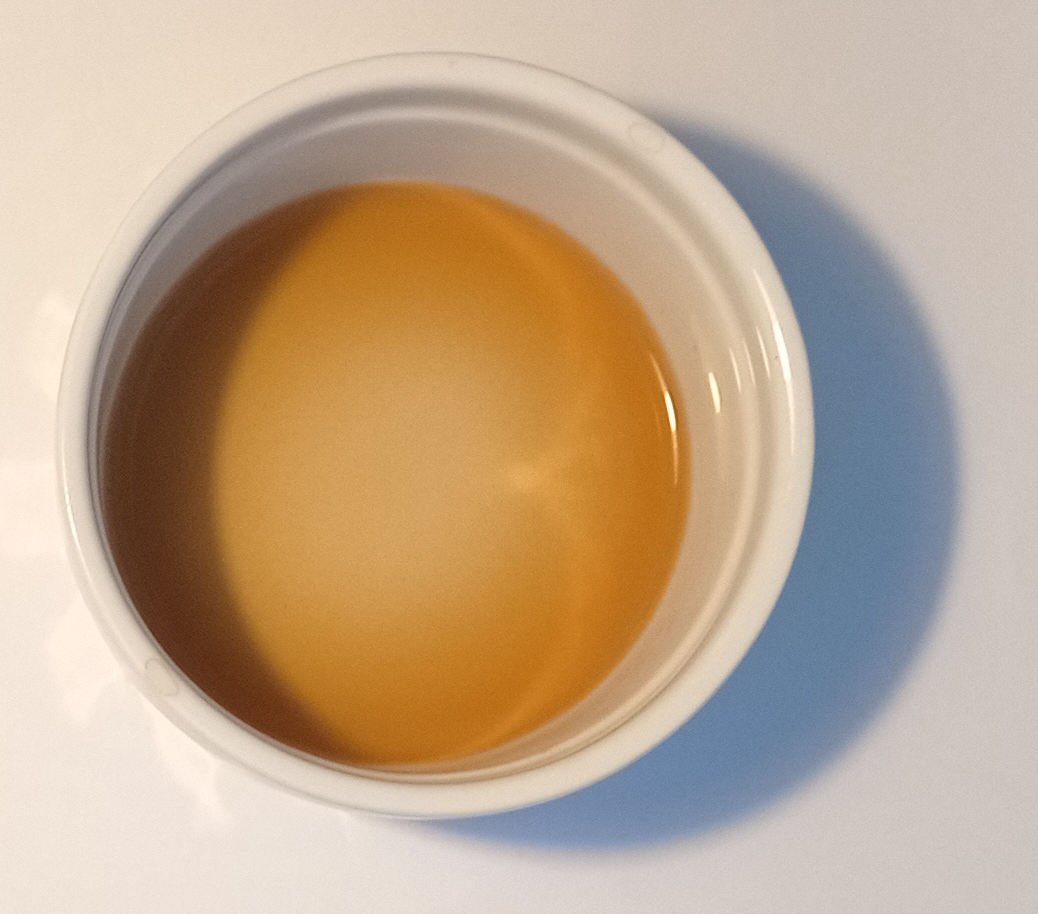
\includegraphics[scale=\myscale,scale=0.17]{figures/caustique}	
\end{minipage}	
\begin{minipage}{0.45\textwidth}  
\myfigure{0.5}{\tikzinput{fig-epicycloide-03}}
\end{minipage}
\end{center}

C'est la courbe visible à la surface du café dans une tasse éclairée par un point éloigné. La caustique correspond aux points où il y a une concentration de lumière. D'un point de vue mathématique et optique, des rayons lumineux parallèles se réfléchissent sur le cercle, la caustique est \emph{l'enveloppe} des rayons réfléchis, c'est-à-dire la courbe tangente aux rayons réfléchis. Ce sont des effets optiques en général très difficiles à calculer, par exemple on ne peut pas les obtenir par \emph{ray-tracing}.

\myfigure{0.7}{\tikzinput{fig-epicycloide-04}}


Sur la figure ci-dessus : une source lumineuse est placée à l'infini à gauche, les rayons lumineux arrivent parallèlement et horizontalement. Regardons la trajectoire du rayon incident\couleurnb{ (orange)}{}, il vient intersecter le demi-cercle et se réfléchit ensuite\couleurnb{ (en bleu)}{} en suivant la loi de réflexion de Descartes. Lorsqu'on fait cela plusieurs fois, les rayons réfléchis dessinent le contour d'une courbe : la caustique.


Considérons un cercle $\mathcal{C}_0$ de rayon $4r$, la caustique de ce cercle a pour équation paramétrique :
$$\vec{OM} = 
\begin{pmatrix}
	3r\cos(\theta) - r\cos\left(3\theta \right)  \\ 
	3r\sin(\theta) - r\sin\left(3\theta \right)
\end{pmatrix} \qquad \theta \in \left[-\frac\pi2, \frac\pi2\right].$$



\end{exemple}


%%%%%%%%%%%%%%%%%%%%%%%%%%%%%%%%%%%%%%%%%%%%%%%%%%%%%%%%%%%%%%%%%%%%%
\section{Nombres complexes et trigonométrie}

\index{nombre complexe}

%--------------------------------------------------------------------
\subsection{Écriture trigonométrique}

\begin{itemize}
	\item Un \defi{nombre complexe} est un couple $(a, b) \in \Rr^2$ que l'on notera $a + \ii b$. 
    
    \item Le nombre complexe $\ii$ vérifie la relation $\ii ^2 = - 1$.

\myfigure{1}{\tikzinput{fig_complexes_01}} 

    \item Le \defi{module} de $z = a + \ii b$ est le réel positif $|z| = \sqrt{a^2 + b^2}$. Il mesure la distance du point $(a,b)$ à l'origine $(0,0)$.
    
    \item 
    Un nombre complexe $z\in\Cc$, admet l'écriture trigonométrique :
    $$z = r\cos(\theta)  + \ii r\sin(\theta) \qquad
    	\text{ avec } \quad r \in\Rr_+ \quad \text{ et } \quad \theta \in \Rr$$
    
    \myfigure{1}{\tikzinput{fig_complexes_06}}
    
    \begin{itemize}
    	\item $r$ est en fait le module de $z$ : $r=|z|$,
    	\item $\theta$ est un \defi{argument} de $z$, on le note $\arg(z)$ (en radians).
    \end{itemize}

   \item Nous définissons la \defi{notation exponentielle} par
   $$e^{\ii  \theta} = \cos(\theta) + \ii  \sin(\theta)$$
   et donc tout nombre complexe s'écrit :
   $$z = r e^{\ii  \theta}$$
   o\`u $r = \left| z \right|$ est son module et $\theta = \arg (z)$ est un de ses arguments.
   
\end{itemize}

%--------------------------------------------------------------------
\subsection{Exemple}


\begin{exemple}
On considère un système composé de deux bras articulés, le premier peut tourner autour d'un point fixe, le second tourne autour de l'extrémité du premier. Comment calculer la position de l'extrémité du second bras ?

\myfigure{0.8}{\tikzinput{fig-linkage}}

Notons $r_1$ et $r_2$ les longueurs (fixes) des deux bras. Les paramètres variables sont les angles $\theta_1$ et $\theta_2$ entre chaque bras et l'horizontale.
Le vecteur $\vec{OM_1}$, et le point $M_1$, ont pour affixe :
$$z_1 = r_1 e^{\ii \theta_1}.$$

Le vecteur $\vec{M_1M_2}$ a pour affixe : 
$$z_2 - z_1 = r_2 e^{\ii \theta_2}.$$

Ainsi le vecteur $\vec{OM_2}$, et le point $M_2$, ont pour affixe :
$$z_2 = r_1 e^{\ii \theta_1} + r_2 e^{\ii \theta_2}.$$
Si on souhaite retourner aux coordonnées $(x,y)$ de $M_2$, ce sont :	
$$\begin{pmatrix}
	r_1\cos(\theta_1) + r_2\cos(\theta_2) \\ 
	r_1\sin(\theta_1) + r_2\sin(\theta_2)
\end{pmatrix}.$$
\end{exemple}


%--------------------------------------------------------------------
\subsection{Transformations géométriques}

Voici quelques transformations élémentaires exprimées à l'aide des nombres complexes.
On identifie un nombre complexe $z = x + \ii y$ avec le point $M(x,y)$ ; ainsi une transformation du plan correspond à une fonction $z \mapsto f(z)$.


\begin{enumerate}
	\item \textbf{Translation.}\index{translation}
	La translation de vecteur $\left(\begin{smallmatrix}a\\b\end{smallmatrix}\right)$ correspond à l'addition du nombre complexe $z_0 = a + \ii b$.
	
	\begin{center}		
	\begin{minipage}{0.45\textwidth}
    $$z \mapsto z + z_0$$
	\end{minipage}
	\begin{minipage}{0.45\textwidth}
		\myfigure{0.4}{\tikzinput{fig-transfo-01}}
	\end{minipage}
	\end{center}

	\item \textbf{Réflexion horizontale.}\index{reflexion@réflexion}
	La réflexion par rapport à l'axe des abscisses correspond à la conjugaison complexe.

	\begin{center}
	\begin{minipage}{0.45\textwidth}
		$$z = x + \ii y \mapsto \bar z = x - \ii y$$
	\end{minipage}
	\begin{minipage}{0.45\textwidth}
		\myfigure{0.4}{\tikzinput{fig-transfo-02}}
	\end{minipage}
	\end{center}

	\item \textbf{Homothétie.}\index{homothetie@homothétie}
   L'homothétie centrée à l'origine et de rapport $r \in \Rr^*$ correspond à la multiplication par le réel $r$.
   
   \begin{center}
	\begin{minipage}{0.45\textwidth}
	$$z \mapsto rz$$	
	\end{minipage}
	\begin{minipage}{0.45\textwidth}
		\myfigure{0.4}{\tikzinput{fig-transfo-03}}
	\end{minipage}	
	\end{center}

	\item \textbf{Rotation.}\index{rotation}
	La rotation de centre l'origine et d'angle $\theta$ correspond à la multiplication par $e^{\ii \theta}$ (un nombre complexe de module $1$).
	
	\begin{center}
	\begin{minipage}{0.45\textwidth}
	$$z \mapsto e^{\ii \theta} z$$	
	\end{minipage}
	\begin{minipage}{0.45\textwidth}
		\myfigure{0.4}{\tikzinput{fig-transfo-04}}
	\end{minipage}
	\end{center}


	\item \textbf{Similitude.}
	Une similitude directe est la composée d'une homothétie et d'une rotation (ici centrées à l'origine). Elle correspond à la multiplication par un nombre complexe quelconque $w = r e^{\ii \theta}$ avec $r>0$, où $r$ est le rapport et $\theta$ l'angle.
	
	\begin{center}
	\begin{minipage}{0.45\textwidth}
		$$z \mapsto w z$$	
	\end{minipage}
	\begin{minipage}{0.45\textwidth}
		\myfigure{0.4}{\tikzinput{fig-transfo-05}}
	\end{minipage}
	\end{center}

	Si on souhaite une similitude centrée en $z_0 = a + \ii b$ alors la transformation est 
	$z = w (z-z_0) + z_0$. 

\end{enumerate}



%%%%%%%%%%%%%%%%%%%%%%%%%%%%%%%%%%%%%%%%%%%%%%%%%%%%%%%%%%%%%%%%%%%%%
\section{Trigonométrie dans l'espace}

%--------------------------------------------------------------------
\subsection{Coordonnées cylindriques}

\index{coordonnees@coordonnées!cylindriques}

Les coordonnées cylindriques $(r,\theta,z)$ sont un autre système de coordonnées que les coordonnées cartésiennes classiques $(x,y,z)$. 
On obtient les coordonnées cartésiennes à partir des coordonnées cylindriques par les formules suivantes :
$$\left\{\begin{array}{rcl}
	x &=& r\cos(\theta) \\
	y &=& r\sin(\theta) \\	
	z &=& z
\end{array}\right.$$

%\commentfigure{
	\myfigure{0.8}{\tikzinput{coord-cylind-01}}
%}

Ces coordonnées sont uniques lorsque $r>0$ et $\theta \in {}]-\pi,\pi[$.
Elles s'apparentent aux coordonnées polaires avec en plus une hauteur $z$. Elles sont particulièrement adaptées lorsque la configuration possède un axe de rotation.
Les formules inverses sont similaires à celles pour les coordonnées polaires :
$$\left\{\begin{array}{rcl}
	r &=& \sqrt{x^2+y^2} \\
	\theta &=&  \arctantwo(y,x) \\
	z &=& z
\end{array}\right.$$



%--------------------------------------------------------------------
\subsection{Coordonnées sphériques}

\index{coordonnees@coordonnées!spheriques@sphériques}

Les coordonnées sphériques $(r, \varphi, \lambda)$ sont la donnée d'une altitude $r$, d'une latitude $\varphi$ et d'une longitude $\lambda$. Elles permettent de se repérer dans l'espace et particulièrement sur une sphère ($r$, son rayon, est alors fixe). Ce sont les coordonnées naturelles des navigateurs.
Le passage des coordonnées sphériques vers les coordonnées cartésiennes s'exprime par :
$$\left\{\begin{array}{rcl}
	x & = & r \cos(\varphi) \cos(\lambda) \\
	y & = & r \cos(\varphi) \sin(\lambda) \\
	z & = & r \sin(\varphi)
\end{array}\right.$$

\commentfigure{
\myfigure{0.8}{\tikzinput{fig-sphere-01}}
}

Ces coordonnées sont uniques si $r>0$, $\varphi \in {}]-\frac\pi2,\frac\pi2[ $, $\lambda \in {}]-\pi,\pi]$.
Attention ! Les notations et les choix d'angles (latitude, colatitude\ldots) diffèrent selon les sources.

Les formules inverses sont :
$$\left\{\begin{array}{rcl}
	r &=& \sqrt{x^2+y^2+z^2} \\	
	\varphi &=& \arcsin\left(\frac z r\right) \\
    \lambda &=& \arctantwo(y,x) \\
\end{array}\right.$$


\end{document}
